\documentclass[reqno]{amsart}


\pagestyle{empty}

\usepackage{graphicx}
\usepackage[margin = 1cm]{geometry}
\usepackage{color}
\usepackage{cancel}
\usepackage{multirow}
\usepackage{framed}
\usepackage{algorithm}
\usepackage{algorithmic}
\usepackage{amssymb}
\usepackage{stackengine}


\newtheorem{thm}{Theorem}
\newtheorem{cor}{Corollary}
\theoremstyle{definition}
\newtheorem{definition}{Definition}

\newenvironment{handwave}{%
  \renewcommand{\proofname}{Handwavey proof}\proof}{\endproof}
  %\renewcommand{\qedsymbol}{$\blacksquare$}

\begin{document}
\begin{flushleft}
{\sc \Large AMATH 301 Rahman} \hfill Week 8 Theory Part 1
\bigskip
\end{flushleft}

\newcommand{\R}{\mathbb{R}}
\newcommand{\N}{\mathbb{N}}
\newcommand{\Z}{\mathbb{Z}}
\newcommand{\Q}{\mathbb{Q}}
\renewcommand{\CancelColor}{\color{red}}
\newcommand{\?}{\stackrel{?}{=}}
\renewcommand{\varphi}{\phi}
\newcommand{\card}{\text{Card}}
\newcommand{\bigzero}{\text{\Huge 0}}
\newcommand{\curvearrowdown}{{\color{red}\rotatebox{90}{$\curvearrowleft$}}}
\newcommand{\curvearrowup}{{\color{red}\rotatebox{90}{$\curvearrowright$}}}



\section*{Week 8 Part 1:  Intro to ODE Modeling}

What is a Differential Equation and why do we study them?

Many things in life ranging from nuclear physics to love affairs involves changes in on quantity in relation to another.  Since
we understand rates of change as ``differentials'' it is natural to model these phenomena as differential equations.

\begin{enumerate}

\item[Ex:  ] Consider carbon dating.  We know that all living things
contain $C_{12}$ and $C_{14}$, however when living things die
the $C_{14}$ starts to decay because it is radioactive.  We can model
this decay.  First let $t$ be the time that has elapsed since the death
of the body.  Also, let $x(t)$ be the amount of $C_{14}$ left after
a period of time $t$.  We know the decay is linear, so our rate of change
will be governed by the following equation,
%
\begin{equation*}
\frac{dx}{dt} = -kx,
\end{equation*}
%
where $k$ is the rate constant.  Basically the $C_{14}$ decay at a rate
of $kx$ [mass/time].

We also discussed direction fields for this problem, which is given bellow.
For the field first calculate $dx/dt = 0$, called the ``equilibrium solution''
or ``fixed point'', which is the easiest solution to
find.  Then after plotting that slope for the respective $x,t$ values find
what the other slopes are for other relevant $x$ and $t$ values.

\begin{figure}[htbp]
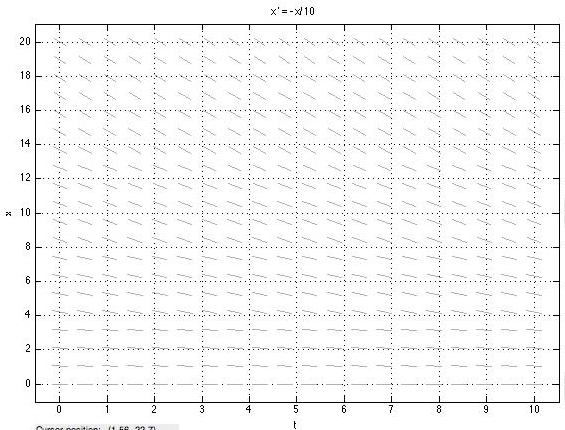
\includegraphics[scale=.42]{DF1.jpg}
\end{figure}

\end{enumerate}

The next example is a very important example that appears on exams frequently.

\begin{enumerate}

\item[Ex:  ]

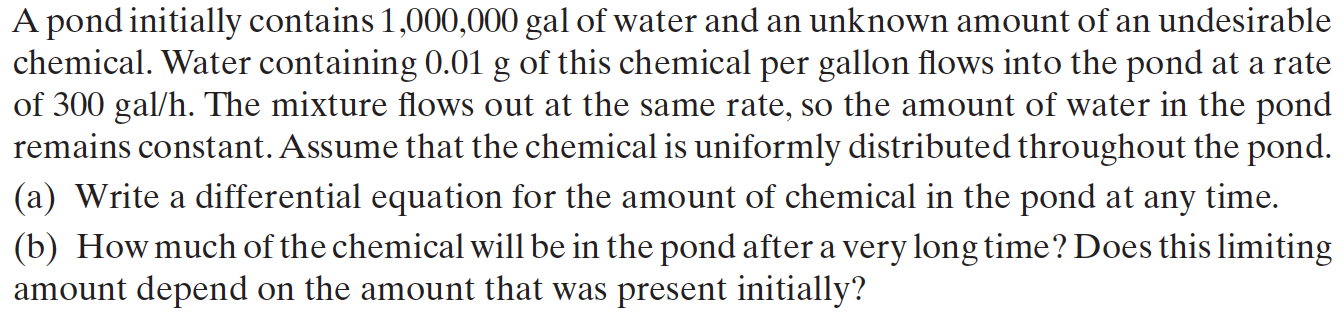
\includegraphics[width = 0.9\textwidth]{BoyceDiPrima_pg9_Ex21}

\textbf{Solution:  }
\begin{enumerate}

\item[a)]  We want to find the rate at which the amount of chemical is changing.
When we develop models one should always keep track of the dimensions.  It
provides you with information and reduces the chance of making a mistake.

Now, let $x(t)$ be the amount of chemical in grams at a time $t$ in hours.
We know that the rate will be $dx/dt$, but to find the model we must realize
that Total Rate = {\color{blue}(Rate in)} - {\color{red}(Rate out)}.  Notice that
{\color{blue}(Rate in) = (.01 g/gal) $\times$ (300 gal/h) = 3 g/h},
and {\color{red}(Rate out) = (300 gal/h) $\times$ (x/(1 Million) g/gal) = (3/1000)x g/h}.  So, our
model becomes,

\begin{equation*}
\frac{dx}{dt} = {\color{blue}3} - {\color{red}(3 \times 10^{-4})x}.
\end{equation*}

\item[b)]  What are they asking for this problem?  They want to know if the amount
of the chemical blows up or converges to something.  To do this we look for an
equilibrium solution,

\begin{equation*}
\frac{dx}{dt} = 3 - (3 \times 10^{-4})x = 0 \Rightarrow x = 10^4.
\end{equation*}

\end{enumerate}

\end{enumerate}

\bigskip

For the next couple of problems we want to find the ODE that gives us the
behavior delineated in the problem.

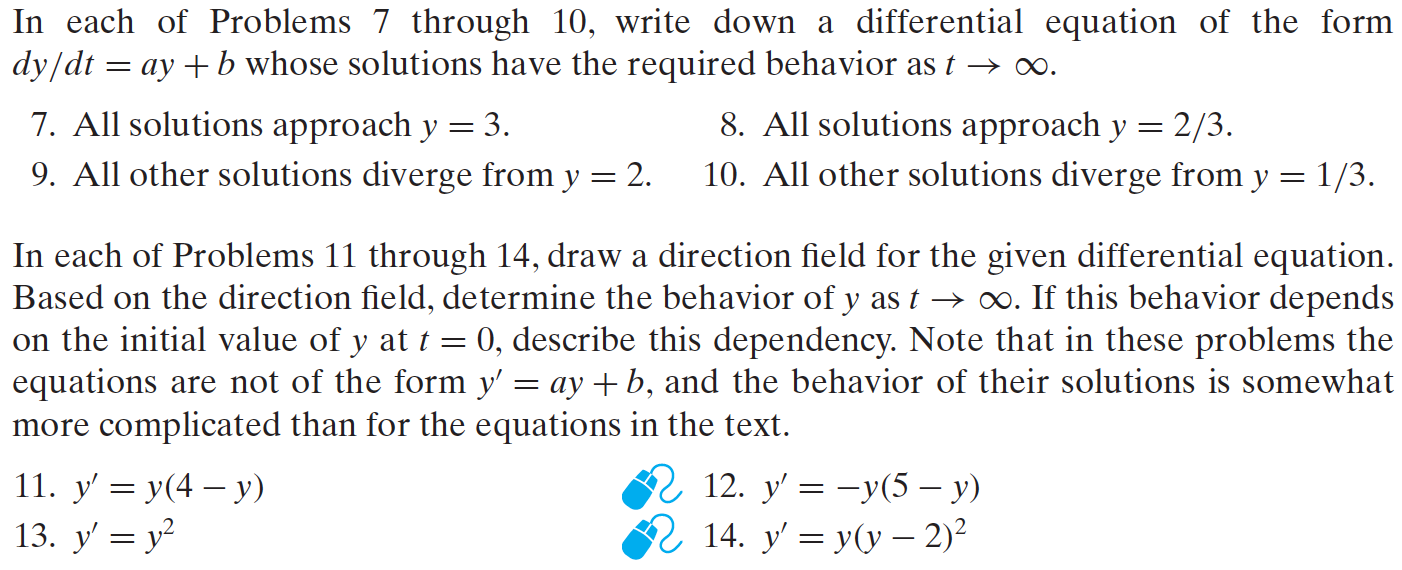
\includegraphics[width = 0.9\textwidth]{BoyceDiPrima_pg9_Ex7to14}

\begin{enumerate}

\item[7)]  $a\cdot 3 + b = 0 \Rightarrow b = -3a$, so in general the equation
will be $y' = -ay + 3a$ since the solutions ``approach''.

\item[9)]  $a\cdot 2 + b = 0 \Rightarrow b = -2a$, so in general the equation
will be $y' = ay - 2a$ since the solutions ``diverge from''.

\end{enumerate}

\bigskip

The next problem is to find the direction field.

\begin{enumerate}

\item[12)]  We first find the equilibrium solutions of $y' = -y(5-y)$, which are
$y_* = 0$ and $y_* = 5$.  To find the ``stability'' of the solutions, which means
whether or not the solution diverges or converges to an equilibrium solution,
we employ the first derivative test.  This gives the following direction field,

\begin{figure}[htbp]
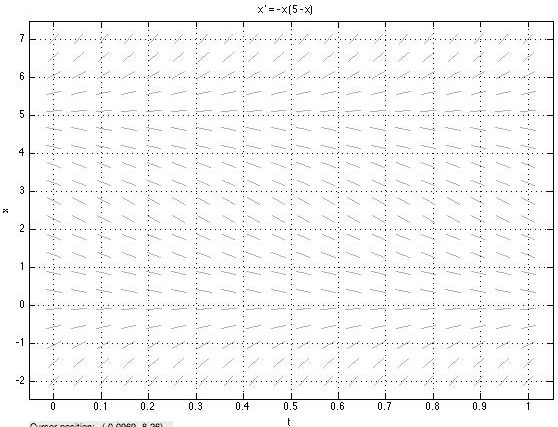
\includegraphics[scale=.42]{DF2.jpg}
\end{figure}

\end{enumerate}


\end{document}